\documentclass[unicode,pdfcover]{hquthesis}
\usepackage{longtable,booktabs}
\usepackage{supertabular}
\usepackage[unicode=false,bookmarks=true,bookmarksnumbered=true,bookmarksopen=false,
 breaklinks=false,pdfborder={0 0 1},backref=false,colorlinks=true]
 {hyperref}

%%%%以下包可根据需要插入，基本涵盖所需内容。
\usepackage{multirow}%画表格推荐先在Excel简单制表，然后复制到该网页{Create LaTeX tables online https://tablesgenerator.com/}自动生成tex代码再粘贴过来（按需进一步简单修改）。
%\usepackage{arydshln}
%\usepackage{amsmath}%公式推荐使用WinEdt 10.3自带的IDE插入，公式外的特殊字符请使用$$ 括起来。
%\usepackage[算法]{algorithm}%算法二字可中文显示“算法”
%\usepackage{algorithmic}
\usepackage{lscape}%横放图表时用到
%\usepackage{longtable}%跨页表格用到

%模拟封面
\title{面向癌症基因数据集的混合协同集成聚类}
\author{李毅}
\supervisor{导师：施一帆 副教授}
\institute{华侨大学工学院}
\date{2026年4月}
\titleEN{Hybrid Collaborative Ensemble Clustering for Cancer Gene Expression Data}
\authoren{Li Yi}
\major{数据科学与大数据技术专业}
\grade{2026}
\studentid{2295141020}
\instituteen{College of Engineering, Huaqiao University}
\majoren{Data Science and Big Data}



\hypersetup{
	pdftitle={面向癌症基因数据集的混合协同集成聚类},
	pdfauthor={李毅},
	pdfsubject={华侨大学学位论文},
	linkcolor=black, anchorcolor=black, citecolor=black,
	filecolor=black, menucolor=black, urlcolor=black
}

\begin{document}
\maketitle

\frontmatter

\begin{abstractCN}
人工智能对癌症基因表达数据的分析很有用。在无监督情况下，集成聚类揭示了基因谱中固有的聚类结构，有助于医学和医疗保健研究的进步。然而，在处理癌症基因数据时，现有的集成聚类方法存在一些局限性：1)噪声特征影响聚类解的生成；2)聚类解的集成忽略了特征子空间；3)统一划分矩阵缺乏优化。在本文中，我们提出了一个用于癌症基因表达数据（HCEC）的混合协作集成聚类框架。首先，HCEC采用多种核化PCA方案提取压缩特征子空间，生成多种聚类方案，减少噪声干扰，从杂交的角度分析基因谱；然后，设计了一种新的共识广泛学习网络，该网络将多个特征子空间和聚类结构信息协同使用，以驱动更好的共识解决方案。通过参数分析、对比实验和消融研究，HCEC的有效性已经在多个真实世界的癌症基因表达数据集上得到了全面的证明。


\end{abstractCN}
\keywordsCN{集成聚类\kwsep 宽度学习系统\kwsep 癌症基因表达\kwsep 核主成分分析\kwsep 医疗人工智能}

\begin{abstractEN}
Artificial intelligence is useful for the analysis of cancer gene expression data. In unsupervised scenario, ensemble clustering uncovers the cluster structure inherent in the gene profiles, which contributes to the advancement of medicine and healthcare research. However, when dealing with cancer gene data, existing ensemble clustering methods have some limitations: 1) the noise features affect the generation of clustering solutions; 2) the integration of clustering solutions ignore the feature subspaces; 3) the unified partition matrix lacks of optimization. In this paper, we propose a hybrid collaborative ensemble clustering framework for cancer gene expression data (HCEC). Firstly, HCEC adopts diverse kernelized PCA schemes to extract compressed feature subspaces and generate multiple clustering solutions, which reduce noise interference and enable the analysis of gene profiles from hybrid perspectives. Then, a novel consensus broad learning network is designed that collaborates multiple feature subspaces and cluster structure information to drive a better consensus solution. Through parameter analysis, comparison experiments, and ablation studies, the effectiveness of HCEC has been comprehensively demonstrated on multiple real-world cancer gene expression datasets.


\end{abstractEN}
\keywordsEN{
	ensemble clustering; broad learning system; cancer gene expression; kernelized PCA; medical artificial intelligence
}


\tableofcontents{}%自动生成章节内容目录，要第二次编译才能生成

%\listoftables%自动生成表格目录，要第二次编译才能生成。如需使用，请去掉前面注释%。若标题含有文献引用，请先注释进行BibTex编译生成bbl文件后，再使用该命令。

%\listoffigures%自动生成图目录，要第二次编译才能生成。如需使用，请去掉前面注释%。若标题含有文献引用，请先注释进行BibTex编译生成bbl文件后，再使用该命令。

\mainmatter

\chapter{绪论}

\section{引言}
引言部分，引言部分，引言部分，引言部分，引言部分，引言部分，引言部分，引言部分，引言部分，引言部分，引言部分，引言部分，引言部分，引言部分，引言部分，引言部分，引言部分，引言部分，引言部分，引言部分，引言部分，引言部分，引言部分，引言部分，引言部分，引言部分，引言部分，引言部分，引言部分，引言部分，引言部分，引言部分，引言部分，引言部分，引言部分，引言部分，引言部分，引言部分，引言部分，引言部分，引言部分，引言部分，引言部分，引言部分，

\section{研究背景与意义}
研究背景与意义，研究背景与意义，研究背景与意义，研究背景与意义，研究背景与意义，研究背景与意义，研究背景与意义，研究背景与意义，研究背景与意义，研究背景与意义，研究背景与意义，研究背景与意义，研究背景与意义，研究背景与意义，研究背景与意义，研究背景与意义，研究背景与意义，研究背景与意义，研究背景与意义，研究背景与意义，研究背景与意义，研究背景与意义，研究背景与意义，研究背景与意义，研究背景与意义，研究背景与意义，研究背景与意义，研究背景与意义，研究背景与意义，研究背景与意义，研究背景与意义，研究背景与意义，研究背景与意义，研究背景与意义，研究背景与意义，研究背景与意义，研究背景与意义，研究背景与意义


\section{本文主要研究内容与贡献}
编译方法：先BibTex一次（编译引用文献Bib文件），再使用XeLaTex连续编译两次。

引言部分，注：一些文献引用示例，引用多个文献\cite{1-1}\cite{1-2}\cite{1-3}，引用期刊文献\cite{1-1}，引用会议文献\cite{2-3}，引用中文文献\cite{1-11}，引用数据集\cite{0-23}等。

图片部分，单一图片如图\ref{fig_papaer_overview}所示
\begin{figure}[tbh]
	\centering
\begin{tabular}{p{14cm}}
	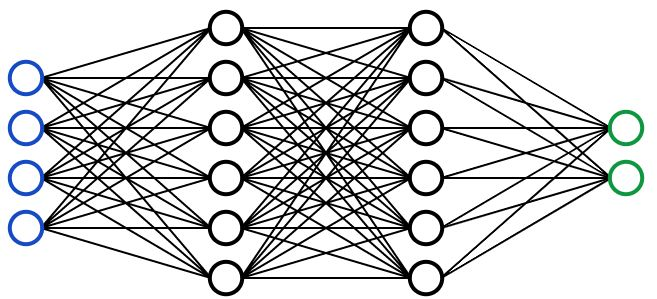
\includegraphics[width=140mm]{./figure/fig_example.png}\\
\end{tabular}
\caption{本文的研究框架}\label{fig_papaer_overview}
\end{figure}

多个图片放置如图\ref{fig_1}所示。
\begin{figure}
  \centering
\begin{tabular}{ccc}
     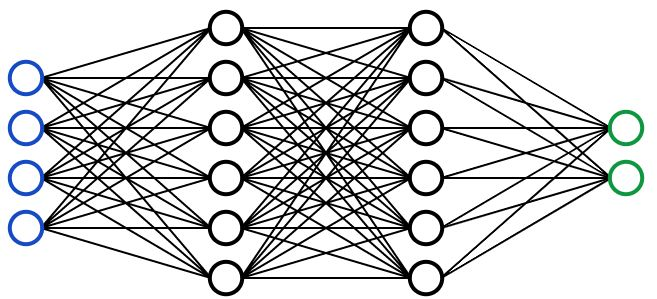
\includegraphics[width=0.45\textwidth]{./figure/fig_example.png}&
     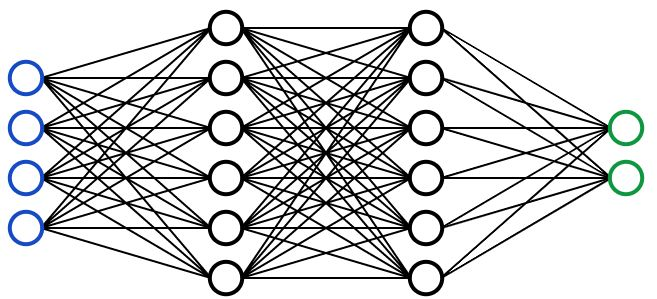
\includegraphics[width=0.45\textwidth]{./figure/fig_example.png}
     \\
     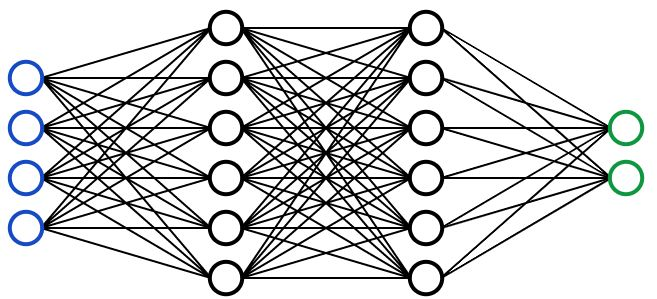
\includegraphics[width=0.45\textwidth]{./figure/fig_example.png}&
     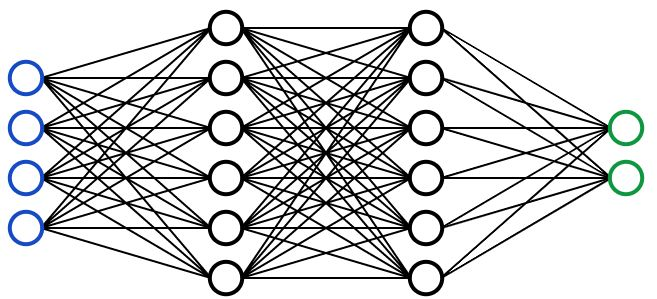
\includegraphics[width=0.45\textwidth]{./figure/fig_example.png}
\end{tabular}
\caption{多个图片放置}
\label{fig_1}
\end{figure}

多个图片加说明的图片放置如图\ref{fig_2}所示
\begin{figure}
\begin{minipage}[t]{0.5\linewidth}
\centering
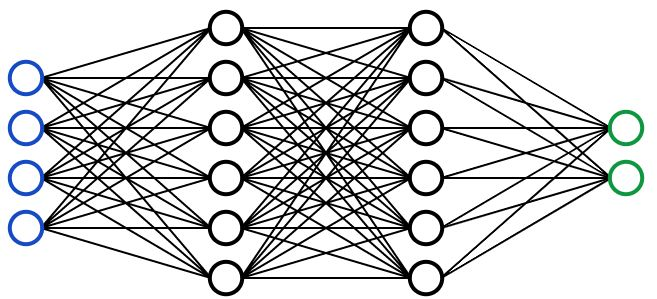
\includegraphics[width=6cm]{./figure/fig_example.png}
\caption*{(A)图片1}
\end{minipage}%
\begin{minipage}[t]{0.5\linewidth}
\centering
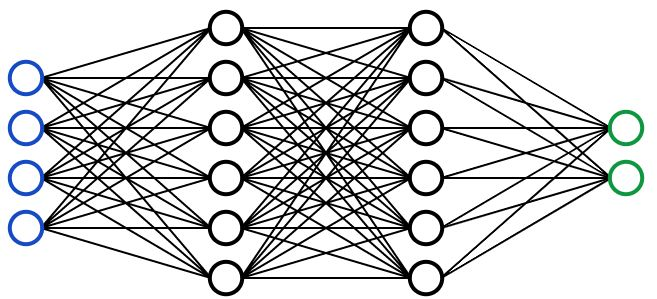
\includegraphics[width=6cm]{./figure/fig_example.png}
\caption*{(B)图片2}
\end{minipage}
\begin{minipage}[t]{0.5\linewidth}
\centering
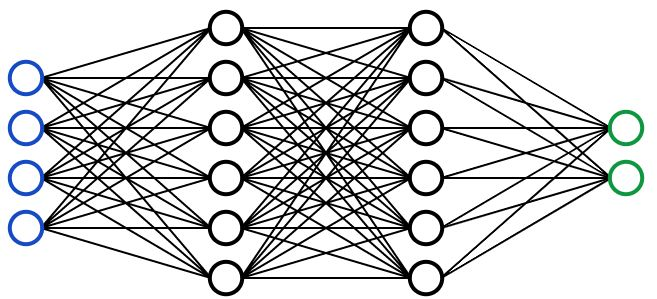
\includegraphics[width=6cm]{./figure/fig_example.png}
\caption*{(C)图片3}
\end{minipage}%
\begin{minipage}[t]{0.5\linewidth}
\centering
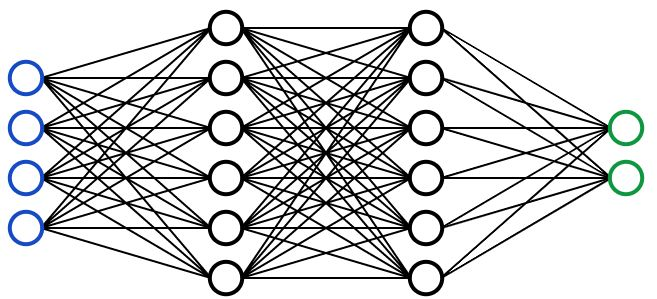
\includegraphics[width=6cm]{./figure/fig_example.png}
\caption*{(D)图片3}
\end{minipage}
\caption{多个图片带说明示例}
\label{fig_2}
\end{figure}


表格写法如表\ref{tab_datasets}所示。
\begin{table}
\caption{实验数据集概述}\label{tab_datasets}
\centering
\begin{tabular} {l l|l l l l}
\hline\hline
$\#$ & 数据集 & $n$ & $d$ & $c$ & 数据领域 \\
\hline
D1 & Movement-libras & 360 & 90 & 15 & 模式识别\\
D2 & Syntheticcontrol & 600 & 60 & 6 & 模式识别\\
D3 & Leaf & 340 & 15 & 36 & 物品图像\\
D4 & Cnae-9 & 1080 & 856 & 9 & 文本分析\\
D5 & Faults & 1941 & 27 & 7 & 模式识别\\
D6 & Mfeat & 2000 & 649 & 10 & 手写数字\\
D7 & Semeion & 1593 & 256 & 10 & 手写数字\\
\hline\hline
\end{tabular}
\end{table}


公式写法如公式(\ref{eq_1})所示。
\begin{equation}
A = B+C=d
\label{eq_1}
\end{equation}


算法写法不固定，如算法\ref{alg_1}可做参考。
\begin{table}
\centering
\caption{算法1的伪代码}
\label{alg_1}
\begin{tabular}{l}
\hline\hline
输入: 数据集$\textbf{X}$，权重参数$\alpha$和$\gamma$ \\
\hline
过程: \\
01: 初始化随机矩阵$W$;\\
02: \textbf{Repeat}\\
03: ~~~~基于公式更新$G$;\\
04: ~~~~基于公式计算$A$;\\
05: \textbf{Until} 公式收敛 \\
06: 得到矩阵$M=(S+S^\mathsf{T})$; \\
\hline
输出: 矩阵$M$ \\
\hline\hline
\end{tabular}
\end{table}




\section{论文结构}

\begin{figure}[tbh]
	\centering
\begin{tabular}{p{14cm}}
	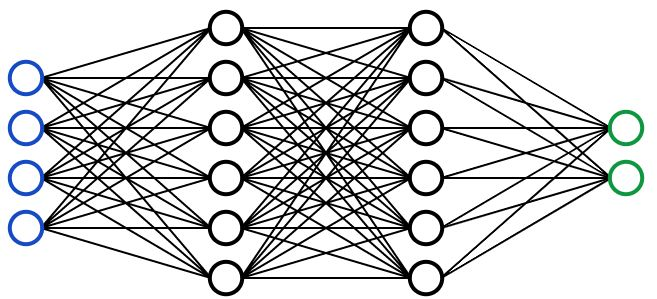
\includegraphics[width=140mm]{./figure/fig_example.png}\\
\end{tabular}
\caption{本文的整体结构}\label{fig_paper_structure}
\end{figure}

本文共由5个章节组成，论文结构如图\ref{fig_paper_structure}所示，各章节具体内容如下：

第一章是绪论，绪论部分内容绪论部分内容绪论部分内容绪论部分内容绪论部分绪论部分内容，绪论部分内容绪论部分内容绪论部分内容绪论部分内容，绪论部分内容绪论部分内容绪论部分内容绪论部分内容绪论部分内容绪论部分内容绪论部分内容，绪论部分内容绪论部分内容

第二章是与本文研究的相关理论与技术的介绍。本文研究的相关理论与技术的介绍，本文研究的相关理论与技术的介绍本文研究的相关理论与技术的介绍，本文研究的相关理论与技术的介绍本文研究的相关理论与技术的介绍本文研究的相关理论与技术的介绍，

第三章详细介绍了第一个算法。介绍了第一个算法。介绍了第一个算法。介绍了第一个算法。

第四章详细介绍了第二个算法。介绍了第二个算法。介绍了第二个算法。介绍了第二个算法。介绍了第二个算法。

第五章详细介绍了第三个算法。介绍了第三个算法。介绍了第三个算法。介绍了第三个算法。介绍了第三个算法。

最后，是本文的总结，以及对未来研究工作的计划与展望。

\section{本章小结}

本章小结内容，本章小结内容本章小结内容本章小结内容，本章小结内容本章小结内容本章小结内容本章小结内容，本章小结内容本章小结内容本章小结内容本章小结内容本章小结内容本章小结内容，本章小结内容本章小结内容本章小结内容本章小结内容。


\chapter{研究现状综述}
\section{相关技术1}

相关技术1的介绍内容，相关技术1的介绍内容，相关技术1的介绍内容，相关技术1的介绍内容，相关技术1的介绍内容，相关技术1的介绍内容，相关技术1的介绍内容，相关技术1的介绍内容，相关技术1的介绍内容，相关技术1的介绍内容，相关技术1的介绍内容，相关技术1的介绍内容，相关技术1的介绍内容，相关技术1的介绍内容，相关技术1的介绍内容，相关技术1的介绍内容，相关技术1的介绍内容，相关技术1 的介绍内容，相关技术1的介绍内容，相关技术1的介绍内容，相关技术1的介绍内容，相关技术1的介绍内容，相关技术1的介绍内容，相关技术1的介绍内容，相关技术1的介绍内容，相关技术1的介绍内容，相关技术1的介绍内容，相关技术1的介绍内容，相关技术1的介绍内容，相关技术1的介绍内容，相关技术1的介绍内容，相关技术1的介绍内容，相关技术1的介绍内容，相关技术1的介绍内容，相关技术1的介绍内容，相关技术1的介绍内容，相关技术1的介绍内容，相关技术1的介绍内容，相关技术1的介绍内容，相关技术1的介绍内容，相关技术1的介绍内容，相关技术1的介绍内容，相关技术1的介绍内容，相关技术1的介绍内容，相关技术1的介绍内容，相关技术1的介绍内容，相关技术1的介绍内容，相关技术1的介绍内容，相关技术1的介绍内容，相关技术1的介绍内容，相关技术1的介绍内容，相关技术1的介绍内容，相关技术1的介绍内容，相关技术1的介绍内容，相关技术1的介绍内容，相关技术1的介绍内容，相关技术1的介绍内容，相关技术1的介绍内容，相关技术1的介绍内容，相关技术1的介绍内容，

相关技术1的介绍内容，相关技术1的介绍内容，相关技术1的介绍内容，相关技术1的介绍内容，相关技术1的介绍内容，相关技术1的介绍内容，相关技术1的介绍内容，相关技术1的介绍内容，相关技术1的介绍内容，相关技术1的介绍内容，相关技术1的介绍内容，相关技术1的介绍内容，相关技术1的介绍内容，相关技术1的介绍内容，相关技术1的介绍内容，相关技术1的介绍内容，相关技术1的介绍内容，相关技术1的介绍内容，相关技术1的介绍内容，相关技术1的介绍内容，相关技术1的介绍内容，相关技术1的介绍内容，相关技术1的介绍内容，相关技术1的介绍内容，


\section{相关技术2}

相关技术2的介绍内容，相关技术2的介绍内容，相关技术2的介绍内容，相关技术2的介绍内容，相关技术2的介绍内容，相关技术2的介绍内容，相关技术2的介绍内容，相关技术2的介绍内容，相关技术2的介绍内容，相关技术2的介绍内容，相关技术2的介绍内容，相关技术2的介绍内容，相关技术2的介绍内容，相关技术2的介绍内容，相关技术2的介绍内容，相关技术2的介绍内容，相关技术2的介绍内容，相关技术2 的介绍内容，相关技术2的介绍内容，相关技术2的介绍内容，相关技术2的介绍内容，相关技术2的介绍内容，相关技术2的介绍内容，相关技术2的介绍内容，相关技术2的介绍内容，相关技术2的介绍内容，相关技术2的介绍内容，相关技术2的介绍内容，相关技术2的介绍内容，相关技术2的介绍内容，相关技术2的介绍内容，相关技术2的介绍内容，相关技术2的介绍内容，相关技术2的介绍内容，相关技术2的介绍内容，相关技术2的介绍内容，相关技术2的介绍内容，相关技术2的介绍内容，相关技术2的介绍内容，相关技术2的介绍内容，相关技术2的介绍内容，相关技术2的介绍内容，相关技术2的介绍内容，相关技术2的介绍内容，相关技术2的介绍内容，相关技术2的介绍内容，相关技术2的介绍内容，相关技术2的介绍内容，




\chapter{面向癌症基因数据集的混合协同集成聚类}

\section{概述}
本章的概述内容，本章的概述内容，本章的概述内容，本章的概述内容，本章的概述内容，本章的概述内容，本章的概述内容，本章的概述内容，本章的概述内容，本章的概述内容，本章的概述内容，本章的概述内容，本章的概述内容，本章的概述内容，本章的概述内容，本章的概述内容，本章的概述内容，本章的概述内容，本章的概述内容，本章的概述内容，本章的概述内容，本章的概述内容，本章的概述内容，本章的概述内容，本章的概述内容，本章的概述内容，本章的概述内容，本章的概述内容，本章的概述内容，本章的概述内容，本章的概述内容，本章的概述内容，本章的概述内容，本章的概述内容，本章的概述内容，本章的概述内容，本章的概述内容，本章的概述内容，本章的概述内容，本章的概述内容，本章的概述内容，本章的概述内容，

\section{第一章第一节}

\subsection{子节1}

本章第一节子节1的内容，本章第一节子节1的内容，本章第一节子节1的内容，本章第一节子节1的内容，本章第一节子节1的内容，本章第一节子节1的内容，本章第一节子节1的内容，本章第一节子节1的内容，本章第一节子节1的内容，本章第一节子节1的内容，本章第一节子节1的内容，本章第一节子节1的内容，本章第一节子节1的内容，本章第一节子节1的内容，本章第一节子节1的内容，本章第一节子节1的内容，本章第一节子节1的内容，本章第一节子节1的内容，本章第一节子节1的内容，本章第一节子节1的内容，本章第一节子节1的内容，本章第一节子节1的内容，本章第一节子节1的内容，本章第一节子节1 的内容，本章第一节子节1的内容，本章第一节子节1的内容，本章第一节子节1的内容，本章第一节子节1的内容，本章第一节子节1的内容，本章第一节子节1的内容，本章第一节子节1的内容，本章第一节子节1的内容，本章第一节子节1的内容，本章第一节子节1的内容，本章第一节子节1的内容，本章第一节子节1的内容，本章第一节子节1的内容，本章第一节子节1的内容，本章第一节子节1的内容，本章第一节子节1的内容，本章第一节子节1的内容，本章第一节子节1的内容，本章第一节子节1的内容，本章第一节子节1的内容，

\subsection{子节2}

本章第一节子节2的内容，本章第一节子节2的内容，本章第一节子节2的内容，本章第一节子节2的内容，本章第一节子节2的内容，本章第一节子节2的内容，本章第一节子节2的内容，本章第一节子节2的内容，本章第一节子节2的内容，本章第一节子节2的内容，本章第一节子节2的内容，本章第一节子节2的内容，本章第一节子节2的内容，本章第一节子节2的内容，本章第一节子节2的内容，本章第一节子节2的内容，本章第一节子节2的内容，本章第一节子节2的内容，本章第一节子节2的内容，本章第一节子节2的内容，本章第一节子节2的内容，本章第一节子节2的内容，本章第一节子节2的内容，本章第一节子节2的内容，本章第一节子节2的内容，本章第一节子节2的内容，

\section{时间复杂度分析}

本章算法时间复杂度分析，本章算法时间复杂度分析，本章算法时间复杂度分析，本章算法时间复杂度分析，本章算法时间复杂度分析，本章算法时间复杂度分析，本章算法时间复杂度分析，本章算法时间复杂度分析，本章算法时间复杂度分析，本章算法时间复杂度分析，本章算法时间复杂度分析，本章算法时间复杂度分析，本章算法时间复杂度分析，本章算法时间复杂度分析，本章算法时间复杂度分析，本章算法时间复杂度分析，本章算法时间复杂度分析，本章算法时间复杂度分析，本章算法时间复杂度分析，本章算法时间复杂度分析，本章算法时间复杂度分析，本章算法时间复杂度分析，本章算法时间复杂度分析，本章算法时间复杂度分析，

\section{实验}

本章算法实验部分，本章算法实验部分，本章算法实验部分，本章算法实验部分，本章算法实验部分，本章算法实验部分，本章算法实验部分，本章算法实验部分，本章算法实验部分，本章算法实验部分，本章算法实验部分，本章算法实验部分，本章算法实验部分，本章算法实验部分，本章算法实验部分，本章算法实验部分，本章算法实验部分，本章算法实验部分，本章算法实验部分，本章算法实验部分，本章算法实验部分，本章算法实验部分，本章算法实验部分，本章算法实验部分，本章算法实验部分，本章算法实验部分，本章算法实验部分，本章算法实验部分，本章算法实验部分，本章算法实验部分，本章算法实验部分，本章算法实验部分，本章算法实验部分，本章算法实验部分，本章算法实验部分，本章算法实验部分，本章算法实验部分，本章算法实验部分，本章算法实验部分，本章算法实验部分，本章算法实验部分，本章算法实验部分，本章算法实验部分，本章算法实验部分，本章算法实验部分，本章算法实验部分，本章算法实验部分，本章算法实验部分，本章算法实验部分，本章算法实验部分，本章算法实验部分，本章算法实验部分，本章算法实验部分，本章算法实验部分，本章算法实验部分，本章算法实验部分，本章算法实验部分，本章算法实验部分，本章算法实验部分，本章算法实验部分，

\section{本章小结}

本章内容小结，本章内容小结，本章内容小结，本章内容小结，本章内容小结，本章内容小结，本章内容小结，本章内容小结，本章内容小结，本章内容小结，本章内容小结，本章内容小结，本章内容小结，本章内容小结，本章内容小结，本章内容小结，本章内容小结，本章内容小结，本章内容小结，本章内容小结，本章内容小结，本章内容小结，本章内容小结，本章内容小结，本章内容小结，本章内容小结，本章内容小结，本章内容小结，本章内容小结，本章内容小结，本章内容小结，本章内容小结，本章内容小结，本章内容小结，本章内容小结，本章内容小结，本章内容小结，本章内容小结，本章内容小结，本章内容小结，本章内容小结，本章内容小结，本章内容小结，本章内容小结，本章内容小结，本章内容小结，本章内容小结，本章内容小结，本章内容小结，本章内容小结，本章内容小结，本章内容小结，本章内容小结，本章内容小结，本章内容小结，本章内容小结，本章内容小结，本章内容小结，本章内容小结，本章内容小结，本章内容小结，本章内容小结，本章内容小结，本章内容小结，本章内容小结，本章内容小结，本章内容小结，本章内容小结，本章内容小结，本章内容小结，本章内容小结，本章内容小结，本章内容小结，本章内容小结，本章内容小结，




\chapter{实验}

\section{概述}
第二章的概述第二章的概述第二章的概述第二章的概述第二章的概述第二章的概述第二章的概述第二章的概述第二章的概述第二章的概述第二章的概述第二章的概述第二章的概述第二章的概述第二章的概述第二章的概述第二章的概述第二章的概述第二章的概述第二章的概述第二章的概述第二章的概述第二章的概述第二章的概述第二章的概述第二章的概述第二章的概述第二章的概述第二章的概述第二章的概述第二章的概述第二章的概述第二章的概述第二章的概述第二章的概述第二章的概述第二章的概述第二章的概述第二章的概述第二章的概述第二章的概述第二章的概述第二章的概述第二章的概述第二章的概述第二章的概述第二章的概述第二章的概述第二章的概述第二章的概述第二章的概述第二章的概述第二章的概述第二章的概述第二章的概述第二章的概述第二章的概述第二章的概述第二章的概述第二章的概述第二章的概述第二章的概述第二章的概述第二章的概述第二章的概述第二章的概述第二章的概述第二章的概述

\section{第二章第一节}

\subsection{子节1}

第二章第一节子节1的内容，第二章第一节子节1的内容，第二章第一节子节1的内容，第二章第一节子节1的内容，第二章第一节子节1的内容，第二章第一节子节1的内容，第二章第一节子节1的内容，第二章第一节子节1的内容，第二章第一节子节1的内容，第二章第一节子节1的内容，第二章第一节子节1的内容，第二章第一节子节1的内容，第二章第一节子节1的内容，第二章第一节子节1的内容，第二章第一节子节1的内容，第二章第一节子节1的内容，第二章第一节子节1的内容，第二章第一节子节1的内容，第二章第一节子节1的内容，第二章第一节子节1的内容，第二章第一节子节1的内容，第二章第一节子节1的内容，第二章第一节子节1的内容，第二章第一节子节1的内容，第二章第一节子节1的内容，第二章第一节子节1的内容，第二章第一节子节1的内容，第二章第一节子节1的内容，第二章第一节子节1的内容，第二章第一节子节1的内容，第二章第一节子节1的内容，第二章第一节子节1的内容，第二章第一节子节1的内容，第二章第一节子节1的内容，第二章第一节子节1的内容，第二章第一节子节1的内容，第二章第一节子节1的内容，第二章第一节子节1的内容，第二章第一节子节1的内容，第二章第一节子节1的内容

第二章第一节子节1的内容，第二章第一节子节1的内容，第二章第一节子节1的内容，第二章第一节子节1的内容，第二章第一节子节1的内容，第二章第一节子节1的内容，第二章第一节子节1的内容，第二章第一节子节1的内容，第二章第一节子节1的内容，第二章第一节子节1的内容，第二章第一节子节1的内容，第二章第一节子节1的内容，第二章第一节子节1的内容，第二章第一节子节1的内容，第二章第一节子节

\subsection{子节2}

第二章第一节子节2的内容，第二章第一节子节2的内容，第二章第一节子节2的内容，第二章第一节子节2的内容，第二章第一节子节2的内容，第二章第一节子节2的内容，第二章第一节子节2的内容，第二章第一节子节2的内容，第二章第一节子节2的内容，第二章第一节子节2的内容，第二章第一节子节2的内容，第二章第一节子节2的内容，第二章第一节子节2的内容，第二章第一节子节2的内容，第二章第一节子节2的内容，第二章第一节子节2的内容，第二章第一节子节2的内容，第二章第一节子节2的内容，

\section{时间复杂度分析}

第二章算法时间复杂度分析，第二章算法时间复杂度分析，第二章算法时间复杂度分析，第二章算法时间复杂度分析，第二章算法时间复杂度分析，第二章算法时间复杂度分析，第二章算法时间复杂度分析，第二章算法时间复杂度分析，第二章算法时间复杂度分析，第二章算法时间复杂度分析，第二章算法时间复杂度分析，第二章算法时间复杂度分析，第二章算法时间复杂度分析，第二章算法时间复杂度分析，第二章算法时间复杂度分析，第二章算法时间复杂度分析，

\section{实验}
第二章实验部分内容，第二章实验部分内容，第二章实验部分内容，第二章实验部分内容，第二章实验部分内容，第二章实验部分内容，第二章实验部分内容，第二章实验部分内容，第二章实验部分内容，第二章实验部分内容，第二章实验部分内容，第二章实验部分内容，第二章实验部分内容，第二章实验部分内容，第二章实验部分内容，第二章实验部分内容，第二章实验部分内容，第二章实验部分内容，第二章实验部分内容，第二章实验部分内容，

\section{本章小结}

第二章本章小结，第二章本章小结第二章本章小结第二章本章小结，第二章本章小结第二章本章小结第二章本章小结，第二章本章小结第二章本章小结第二章本章小结，第二章本章小结第二章本章小结第二章本章小结，第二章本章小结第二章本章小结第二章本章小结，第二章本章小结第二章本章小结第二章本章小结，第二章本章小结第二章本章小结第二章本章小结，第二章本章小结第二章本章小结第二章本章小结，第二章本章小结第二章本章小结第二章本章小结，第二章本章小结第二章本章小结第二章本章小结，第二章本章小结第二章本章小结第二章本章小结，第二章本章小结第二章本章小结第二章本章小结，第二章本章小结第二章本章小结第二章本章小结，第二章本章小结第二章本章小结第二章本章小结，第二章本章小结第二章本章小结第二章本章小结，第二章本章小结第二章本章小结第二章本章小结，第二章本章小结第二章本章小结第二章本章小结，第二章本章小结第二章本章小结第二章本章小结，第二章本章小结第二章本章小结第二章本章小结，第二章本章小结第二章本章小结第二章本章小结，第二章本章小结第二章本章小结第二章本章小结，第二章本章小结第二章本章小结



\chapter{总结与展望}


全文的内容总结，

（1）全文的内容总结，

（2）全文的内容总结，

（3）全文的内容总结，


\backmatter

%%%%%%%%%%%%%%%%%%%%%%%%%%%%%参考文献%%%%%%%%%%%%%%%%%%%%%%%%%%%%%%

\bibliographystyle{hquthesis}%参考文献格式文件，hquthesis.bst
\bibliography{reference}%收录参考文献的bib文件，reference.bib，如需要换成


\chapterx{致谢}

论文致谢部分，论文致谢部分，论文致谢部分，论文致谢部分，论文致谢部分，论文致谢部分，论文致谢部分，论文致谢部分，论文致谢部分，论文致谢部分，论文致谢部分，论文致谢部分，论文致谢部分，论文致谢部分，论文致谢部分，论文致谢部分，论文致谢部分，论文致谢部分，论文致谢部分，论文致谢部分，论文致谢部分，论文致谢部分，论文致谢部分，论文致谢部分，论文致谢部分，论文致谢部分，论文致谢部分，论文致谢部分，论文致谢部分，论文致谢部分，论文致谢部分，论文致谢部分，论文致谢部分，论文致谢部分，论文致谢部分，论文致谢部分，论文致谢部分，论文致谢部分，论文致谢部分，论文致谢部分，论文致谢部分，论文致谢部分，论文致谢部分，论文致谢部分，论文致谢部分，论文致谢部分，论文致谢部分，论文致谢部分，论文致谢部分，论文致谢部分，论文致谢部分，论文致谢部分，论文致谢部分，论文致谢部分，论文致谢部分，论文致谢部分，论文致谢部分，论文致谢部分，论文致谢部分，论文致谢部分，论文致谢部分，论文致谢部分，论文致谢部分，论文致谢部分，论文致谢部分，论文致谢部分，论文致谢部分，论文致谢部分，论文致谢部分，论文致谢部分，论文致谢部分，论文致谢部分，论文致谢部分，论文致谢部分，论文致谢部分，论文致谢部分，论文致谢部分，论文致谢部分，论文致谢部分，论文致谢部分，论文致谢部分，论文致谢部分，论文致谢部分，论文致谢部分，论文致谢部分，

~\\

\begin{minipage}[t]{0.945\textwidth}%
\begin{flushright}
李毅\\
%\today\\
2026年4月21日于华侨大学%可注释删除
\par\end{flushright}
\end{minipage}

\appendix{附录}
%重新设置表、图、公式的序号和格式，否则接着前面的继续编号       added by YYS
\setcounter{table}{0}
\setcounter{figure}{0}
\setcounter{equation}{0}
\renewcommand{\theequation}{\textbf{A}-\arabic{equation}}%格式为A开头加序号，如A-1，A-2
\renewcommand{\thetable}{\textbf{A}-\arabic{table}}%格式为A开头加序号，如A-1，A-2
\renewcommand{\thefigure}{\textbf{A}-\arabic{figure}}%格式为A开头加序号，如A-1，A-2
\section{在读期间获得的科研成果}

(1) 张三获得2019年xxxxx科创奖，排名第一

(2) Zhang S, Li S, Wang W, et al. How to Love Huaqiao University [J]. IEEE Transaction on Image Processing, 2021, 34(7): 1000-1002

(3) 张三，李四，王五. 一种建设好工学院的神奇装置.发明专利（或者实用发明专利），专利号（或者申请号）：xxxx

(4) 张三，李四，王五. 一种自动想念华侨大学的算法. 软件著作权，登记号：xxxx

\section{关于xxx的代码实现}


\section{关于xxx的数学推导}

%

\end{document}
